\documentclass[11pt]{amsart}
\usepackage{geometry}                % See geometry.pdf to learn the layout options. There are lots.
\geometry{letterpaper}                   % ... or a4paper or a5paper or ... 
%\geometry{landscape}                % Activate for for rotated page geometry
%\usepackage[parfill]{parskip}    % Activate to begin paragraphs with an empty line rather than an indent
\usepackage{graphicx}
\usepackage{amssymb}
\usepackage{amsmath}
\usepackage{epstopdf}
\usepackage{times, natbib, bm, url, subfigure}
\DeclareGraphicsRule{.tif}{png}{.png}{`convert #1 `dirname #1`/`basename #1 .tif`.png}

\title{Appendix C: Relative performance of GAM and bootstrap uncertainty estimation in DSM}
\author{David L. Miller \and
M. Louise Burt \and
Eric A. Rexstad \and 
Len Thomas}
%\date{}                                           % Activate to display a given date or no date

\begin{document}
\maketitle


\section{Introduction}

This appendix gives a summary of a series of very simple simulations that were conducted to investigate the properties of the four methods of uncertainty estimation described in the article. These are: moving block bootstrap (MBB; including detection function uncertainty via the delta method), moving block bootstrap with simulated detection function uncertainty (MBB+SDU; new distance generated from the fitted detection function), GAM uncertainty (GAMU; using standard GAM theory including detection function uncertainty via the delta method) and GAM uncertainty with variance propagation (VARPROP).

Three (admittedly very simple) scenarios were tested; each consisted of a density based on a simple pattern. Creating a ``realistic'' scenario (e.g. including many covariates, correlation and so on) is not easy to construct and such a scenario would never encompass all of the possible combinations. As such, we decided to create three simple situations where it would be easy to discover whether there were difficulties with any of the above methods. The \textsf{R} \texttt{WiSP} (available at \url{http://www.ruwpa.st-and.ac.uk/estimating.abundance/WiSP/index.html}) was used to generate samples and the packages \texttt{dsm} and \texttt{Distance} (available from CRAN) were used to calculate the abundance estimates and corresponding confidence intervals.

\section{Scenarios}

The underlying density surfaces are shown in Figure \ref{sim-plots}. For each of these scenarios, the population size was fixed (at 500 or 5000 individuals) and individuals were randomly placed in the survey area according to the density surface with group size generates from a Poisson distribution with mean 3. A grid of 14 transect lines (parallel to the $y$ axis) the ``height'' of the survey area were placed at a random starting point on the $x$ axis. Points were then detected based on a half-normal detection function with a scale parameter of 0.7, the truncation distance was set to 1.

\begin{figure}[htbp]
\begin{center}
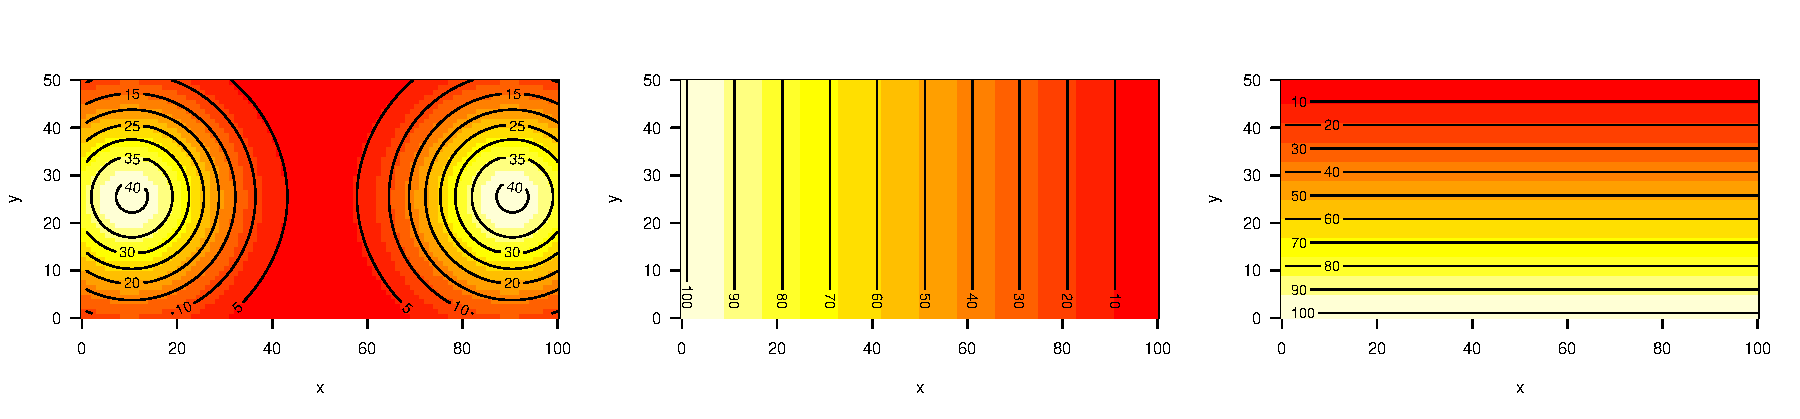
\includegraphics[width=\textwidth]{sim-plots}
\caption{The three underlying density surfaces used in the simulation.}
\label{sim-plots}
\end{center}
\end{figure}

The observations were then allocated to 2 by 2 segments, and a DSM was fitted to the counts. Only a simple bivariate smooth of $x$ and $y$ was fitted to the per-segment counts, a  quasi-Poisson response was used.

Once the model had been fitted, the variance of the predicted abundance was estimated using the four methods listed above. The two moving block bootstraps ran for 200 iterations with a block size of 5.

For each combination of population size and underlying density surface 100 simulations were run. There were no convergence failures.

\section{Results}

\subsection{Population size 5000}

When the true population size in the survey area was 5000, the number of detections was around 900, which seems more than adequate. 

Figure \ref{res-5000} shows the confidence intervals calculated from each of the four methods for each simulation. The left column gives the simulations in order, the right column groups the same results by method. The larger population simulations show that the GAM and variance propagation methods give significantly smaller confidence intervals. 


\begin{figure}
\begin{center}
\setlength{\tabcolsep}{0mm}
\subfigure[]{%
\begin{tabular}{c}
\includegraphics*[width=0.4\textwidth]{results/res-5000-1-1.pdf}\\
\includegraphics*[width=0.4\textwidth]{results/res-5000-2-1.pdf}\\
\includegraphics*[width=0.4\textwidth]{results/res-5000-3-1.pdf}
\end{tabular}
}%
\subfigure[]{%
\begin{tabular}{c}
\includegraphics*[width=0.4\textwidth]{results/res-5000-1-2.pdf}\\
\includegraphics*[width=0.4\textwidth]{results/res-5000-2-2.pdf}\\
\includegraphics*[width=0.4\textwidth]{results/res-5000-3-2.pdf}
\end{tabular}
}%
\caption{Results of simulating populations of 5000 individuals in three scenarios (going down the page). Each coloured horizontal line indicates one simulation result and the black vertical line is truth. On the left side results are grouped by simulation and the blue lines give the point estimate of the population for a given simulation. On the right grouping is by method and the blue points indicate the corresponding point estimates.}
\label{res-5000}
\end{center}
\end{figure}



\subsection{Population size 500}

For the smaller population size the number of detections was around 90. In this situation, the GAM and variance propagation methods appear to have wider intervals than the bootstrap-based methods, however this does have the side effect that the confidence intervals cover truth more often and in general appear to have less erratic behaviour.


\begin{figure}
\begin{center}
\setlength{\tabcolsep}{0mm}
\subfigure[]{%
\begin{tabular}{c}
\includegraphics*[width=0.4\textwidth]{res-500-1-1.pdf}\\
\includegraphics*[width=0.4\textwidth]{res-500-2-1.pdf}\\
%\includegraphics*[width=0.4\textwidth]{res-500-3-1.pdf}
\end{tabular}
}%
\subfigure[]{%
\begin{tabular}{c}
\includegraphics*[width=0.4\textwidth]{res-500-1-2.pdf}\\
\includegraphics*[width=0.4\textwidth]{res-500-2-2.pdf}\\
%\includegraphics*[width=0.4\textwidth]{res-500-3-2.pdf}
\end{tabular}
}%
\caption{Results of simulating populations of 5000 individuals in three scenarios (going down the page). Each coloured horizontal line indicates one simulation result and the black vertical line is truth. On the left side results are grouped by simulation and the blue lines give the point estimate of the population for a given simulation. On the right grouping is by method and the blue points indicate the corresponding point estimates.}
\label{res-500}
\end{center}
\end{figure}

\section{Conclusion}

Admittedly the simulation is rather simplistic, there is no attempt to incorporate other simulated environmental covariates and only a bivariate smooth of location was used in modelling. However, this set up has shown that when there is a large number of observations the GAM-based methods perform well with tighter confidence intervals and good coverage. In the situation when there are fewer observations, we see that (as one would expect) confidence intervals expand and appear more ``noisy''. It is the moving block bootstrap with simulated detection function uncertainty that appear to suffer the most, being tighter than the other methods but with more chaotic behaviour.

Given the significant difference in time taken to calculate the GAM-based intervals and the bootstraps, it seems highly prudent to use the former especially if it is necessary to obtain uncertainty estimates for a white variety of models in a short period of time.

\bibliography{../dsm-refs.bib}


\end{document}  